% Ejercicio 3 - a)
\paragraph{replace-me-with-a-descriptive-text}\label{subsubsec:ej3-a}
Escribir una rutina que se encargue de limpiar el buffer de vídeo y pintarlo
como indica la figura 8. Tener en cuenta que deben ser escritos de forma
genérica para posteriormente ser completados con información del sistema. Además
considerar estas imágenes como sugerencias, ya que pueden ser modificadas a
gusto según cada grupo mostrando siempre la misma información.
\hruler
La sección del mapa la dividimos en 50x50 casilleros. Cada casillero va a tener un estado como por ejemplo $pisado$, $misil$, etc. De acuerdo al
estado pintamos cada casillero con distintas combinaciones de colores.

La sección del contexto del tanque destruido la \fixme{vos eze}

Mostramos además varios relojes. Cada reloj responde a una variable cuyo valor cicla entre $-$, \textbackslash, $-$, y $/$. Se van actualizando 
con distinta frecuencia.

% Ejercicio 3 - b)
\paragraph{replace-me-with-a-descriptive-text}\label{subsubsec:ej3-b}
Escribir las rutinas encargadas de inicializar el directorio y tablas de páginas
para el kernel (mmu inicializar dir kernel). Se debe generar un directorio de
páginas que mapee, usando identity mapping, las direcciones 0x00000000 a
0x00DC3FFF, como ilustra la figura 5. Además, esta función debe inicializar el
directorio de páginas en la dirección 0x27000 y las tablas de páginas según
muestra la figura 1.
\hruler
%bit ti = 0, significa que lo va a buscar a la gdt

A continuación mostramos el esquema de las estructuras que vamos a utilizar para activar paginación.

\begin{figure}[H]
\begin{center}
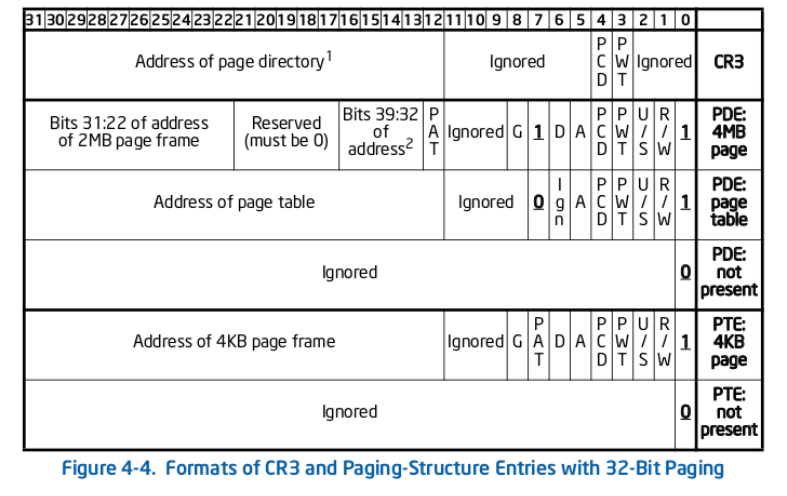
\includegraphics[scale=.5]{imagenes/paginacion.png}
\end{center}
\end{figure}

Vamos a almacenar el page directory en una página en el área de memoria libre, cuyo $address$ vamos a escribir en el registro $cr3$.

En todas las estructuras, vamos a poner:
\begin{itemize}
    \item PCD(Page-Level Cache Disable) = 0 \fixme{explicar estas dos}
    \item PWT(Page-Level Write-Through) = 0
\end{itemize}

El page directory va a tener las primeras cuatro entradas presentes ($p$ = 1) y 1020 no presentes ($p$ = 0). Con estas cuatro entradas del
directorio vamos a poder mapear 4*1024 páginas que es todo lo que precisamos.

Cada uno de estos cuatro directorios va a contener el $address$ de una tabla de páginas que almacenamos en la región de memoria libre.
Los atributos se van a escribir de la siguiente manera:

\fixme{explicar}
\begin{itemize}
    \item G(Global) = 0
    \item PS(Page Size) = 0
    \item A(Accessed) = 0
    \item U/S(User/Supervisor) = 0
    \item R/W(Read/Write) = 1
\end{itemize}

Las tablas de páginas van a tener sus 1024 entradas presentes, con los mismos atributos que las entradas de directorio. Su $address$ va a apuntar
al área de memoria física a la que se éste mapeando.

% Ejercicio 3 - c)
\paragraph{replace-me-with-a-descriptive-text}\label{subsubsec:ej3-c}
Completar el código necesario para activar paginación.
\hruler

Para activar paginación hacemos lo siguiente. Una vez cargado el registro $cr3$ con la dirección del page directory, seteamos el bit más
sigificativo del registro $cr0$.

% Ejercicio 3 - d)
\paragraph{replace-me-with-a-descriptive-text}\label{subsubsec:ej3-d}
Escribir una rutina que imprima el nombre del grupo en pantalla. Debe estar
ubicado en la primer linea de la pantalla alineado a derecha.
\hruler
\fixme{Respuesta}
